\chapter{Assignment: Geolocations}
\label{ch:arheo_geolocations}

The Antikythera data set contains information on the geolocation of artefacts. The location is encoded as \textit{Xsugg}, \textit{Ysugg} coordinates in \textit{epsg:32634} system. We need to transform the data to the more standard \textit{EPSG: 4326} projection, which enables us to see the data on a map. We will do this with the help of a \widget{Python Script}.

\begin{figure}[h]
    \centering
    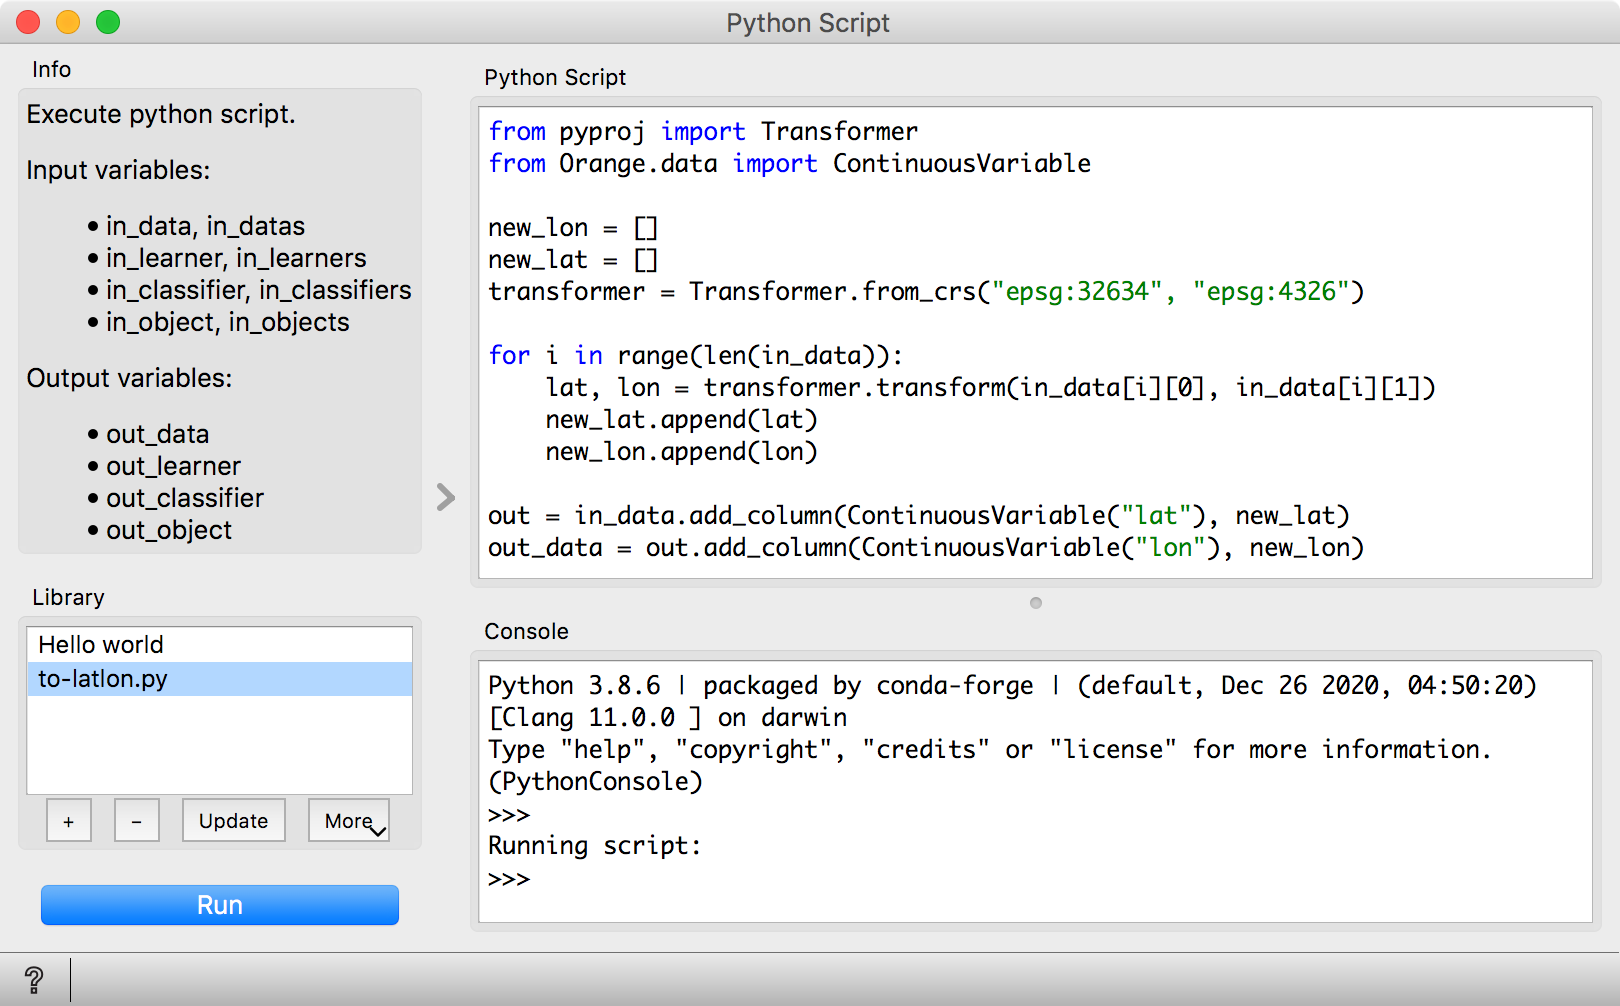
\includegraphics[scale=0.4]{python-script.png}
    \caption{$\;$} % empty caption for proper pagesetting
\end{figure}

\marginnote{For Python Script to work, one needs to have the `pyproj` package installed in the Orange environment. To bypass this, \href{http://file.biolab.si/datasets/pottery.tab}{here} are the preprocessed data you can load with File and connect directly to Geo Map.}

Now, we can plot the data on the map. We will use the Geo add-on for this. If you have not installed the add-on yet, go to Options --> Add-ons and install it. Restart Orange for the add-on to appear.

Connect \widget{Geo Map} to Python Script. The widget should automatically find latitude and longitude attributes, but if it doesn't, you can set them manually. The plot shows where the pottery shards were collected.

\begin{figure}[h]
    \centering
    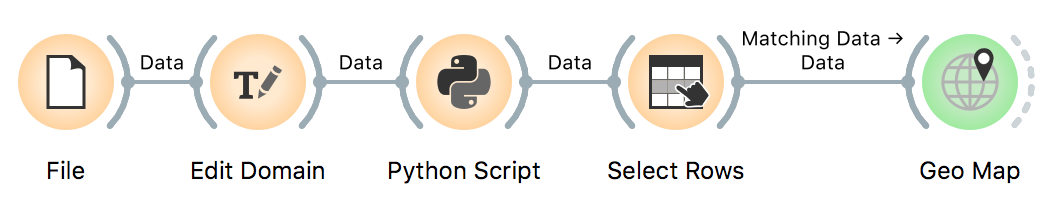
\includegraphics[width=\textwidth]{workflow.png}
    \caption{$\;$} % empty caption for proper pagesetting
\end{figure}

\newpage

\subsection{Assignment}

\begin{figure*}[h]
    \centering
    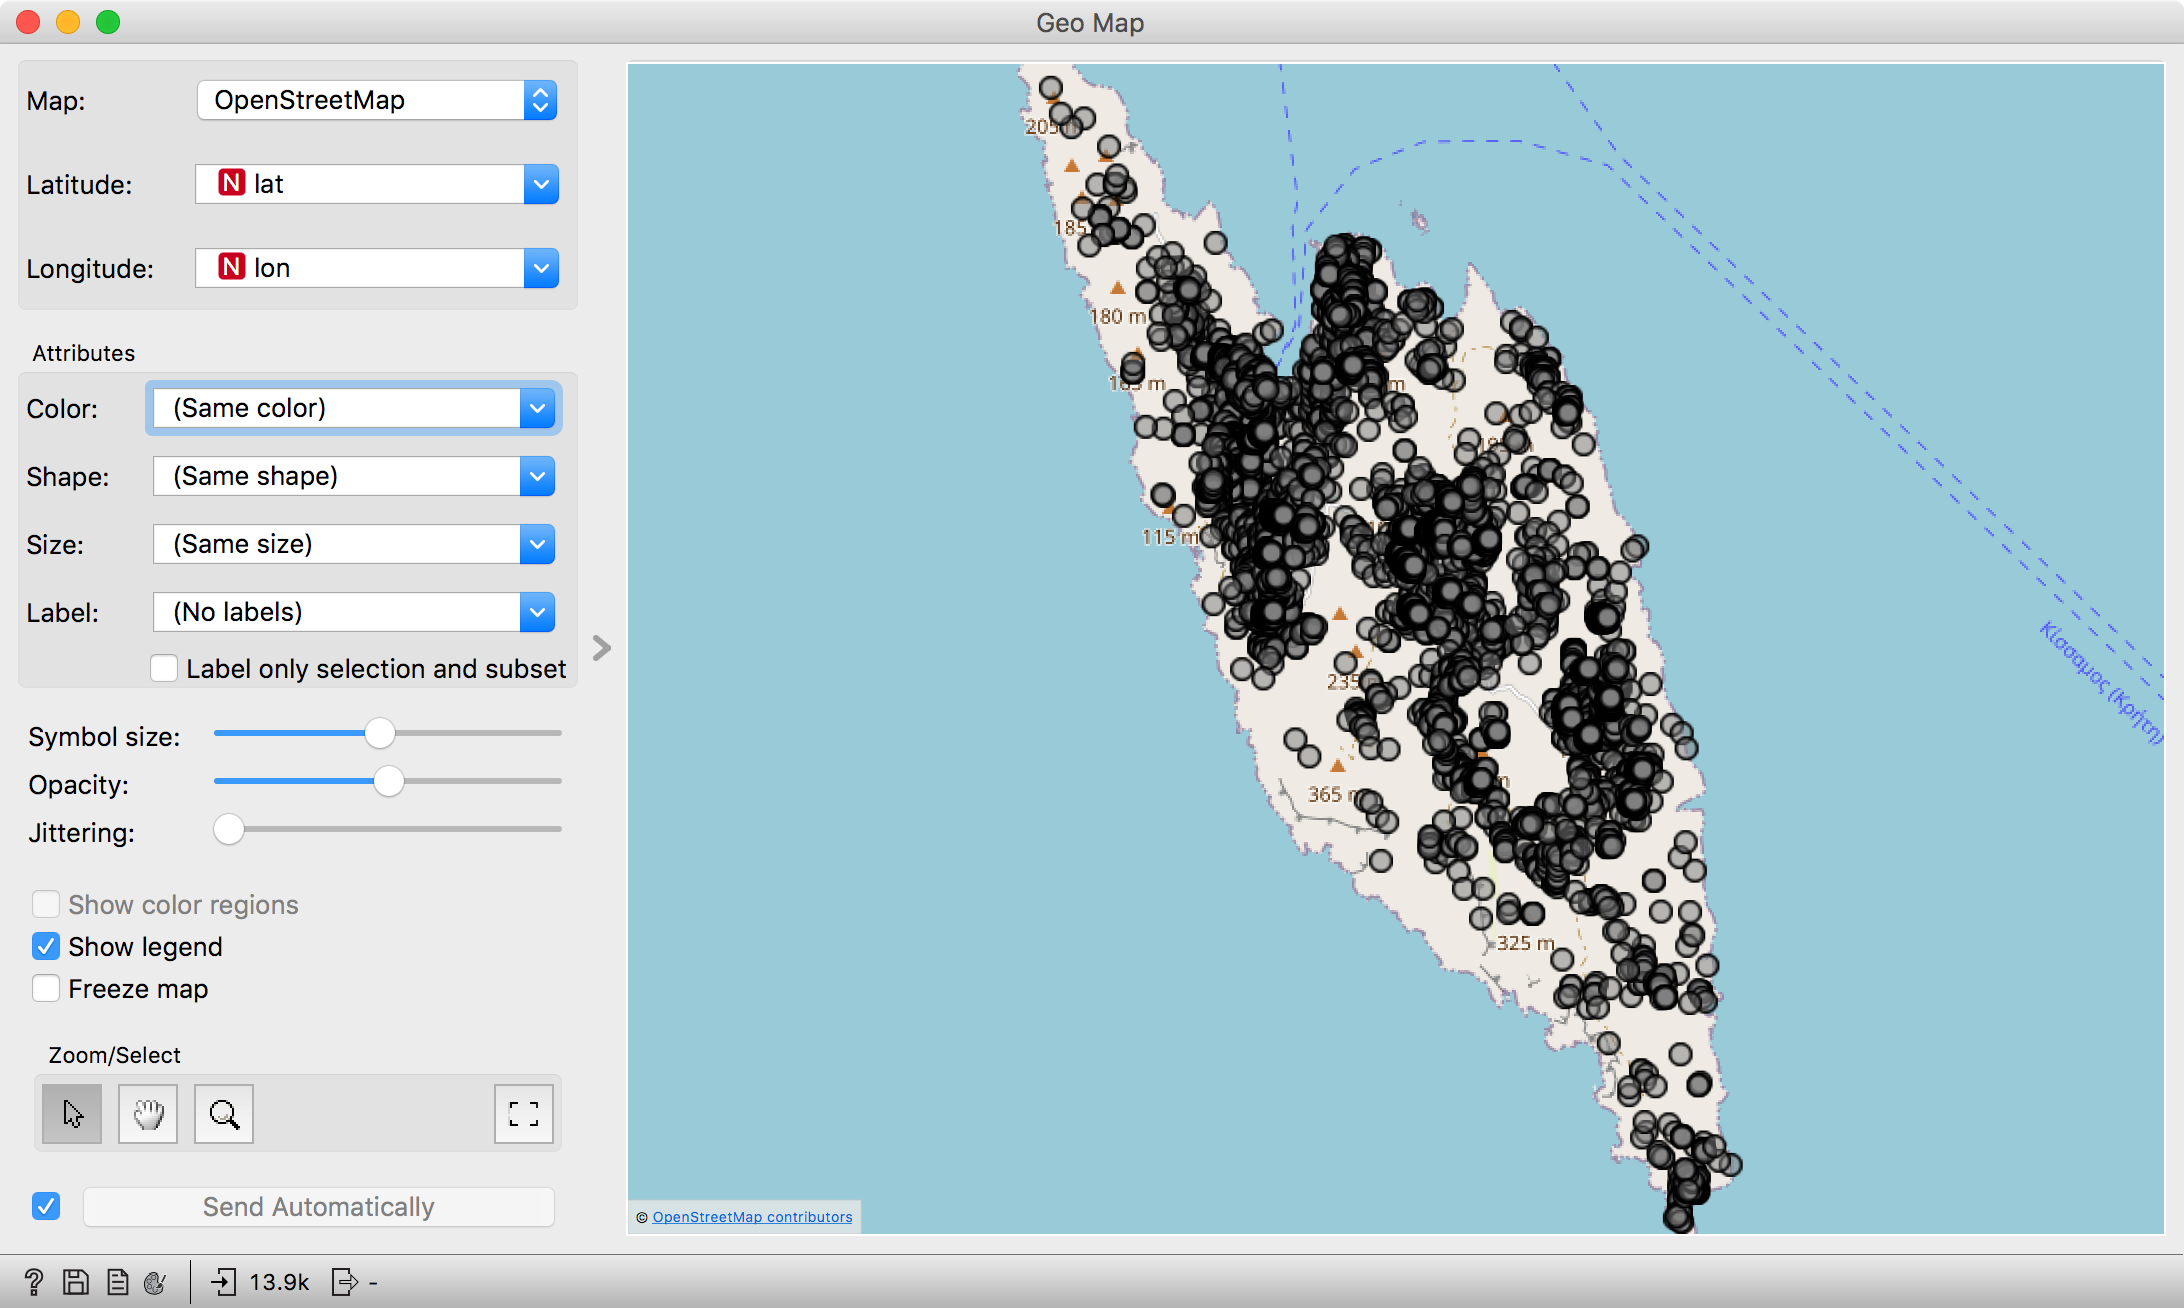
\includegraphics[scale=0.4]{geo-map.png}
    \caption{$\;$} % empty caption for proper pagesetting
\end{figure*}

Use Geo Map widget and color the points by an appropriate attribute to answer the following questions:
\begin{itemize}
    \item Does the location of the shard correspond to the way it was collected?
    \item Use \widget{Select Rows} to keep only data instances with over 75\% certainty that they belong to the a certain period. Go through different periods (attributes from MNLN to Other) and observe if items from one period were found in a specific location of the island. Some periods will produce no results (no items with such high certainty), but that's ok. Skip them.
    \item Use \widget{Select Rows} to explore categorical variables. For example, set the filter to \textit{VesselPart is B} and observe where in the island the shards belonging to the body of the vessel were found. Explore variables of your interest and draw conclusions.
\end{itemize}